\documentclass[1p]{elsarticle_modified}
%\bibliographystyle{elsarticle-num}

%\usepackage[colorlinks]{hyperref}
%\usepackage{abbrmath_seonhwa} %\Abb, \Ascr, \Acal ,\Abf, \Afrak
\usepackage{amsfonts}
\usepackage{amssymb}
\usepackage{amsmath}
\usepackage{amsthm}
\usepackage{scalefnt}
\usepackage{amsbsy}
\usepackage{kotex}
\usepackage{caption}
\usepackage{subfig}
\usepackage{color}
\usepackage{graphicx}
\usepackage{xcolor} %% white, black, red, green, blue, cyan, magenta, yellow
\usepackage{float}
\usepackage{setspace}
\usepackage{hyperref}

\usepackage{tikz}
\usetikzlibrary{arrows}

\usepackage{multirow}
\usepackage{array} % fixed length table
\usepackage{hhline}

%%%%%%%%%%%%%%%%%%%%%
\makeatletter
\renewcommand*\env@matrix[1][\arraystretch]{%
	\edef\arraystretch{#1}%
	\hskip -\arraycolsep
	\let\@ifnextchar\new@ifnextchar
	\array{*\c@MaxMatrixCols c}}
\makeatother %https://tex.stackexchange.com/questions/14071/how-can-i-increase-the-line-spacing-in-a-matrix
%%%%%%%%%%%%%%%

\usepackage[normalem]{ulem}

\newcommand{\msout}[1]{\ifmmode\text{\sout{\ensuremath{#1}}}\else\sout{#1}\fi}
%SOURCE: \msout is \stkout macro in https://tex.stackexchange.com/questions/20609/strikeout-in-math-mode

\newcommand{\cancel}[1]{
	\ifmmode
	{\color{red}\msout{#1}}
	\else
	{\color{red}\sout{#1}}
	\fi
}

\newcommand{\add}[1]{
	{\color{blue}\uwave{#1}}
}

\newcommand{\replace}[2]{
	\ifmmode
	{\color{red}\msout{#1}}{\color{blue}\uwave{#2}}
	\else
	{\color{red}\sout{#1}}{\color{blue}\uwave{#2}}
	\fi
}

\newcommand{\Sol}{\mathcal{S}} %segment
\newcommand{\D}{D} %diagram
\newcommand{\A}{\mathcal{A}} %arc


%%%%%%%%%%%%%%%%%%%%%%%%%%%%%5 test

\def\sl{\operatorname{\textup{SL}}(2,\Cbb)}
\def\psl{\operatorname{\textup{PSL}}(2,\Cbb)}
\def\quan{\mkern 1mu \triangleright \mkern 1mu}

\theoremstyle{definition}
\newtheorem{thm}{Theorem}[section]
\newtheorem{prop}[thm]{Proposition}
\newtheorem{lem}[thm]{Lemma}
\newtheorem{ques}[thm]{Question}
\newtheorem{cor}[thm]{Corollary}
\newtheorem{defn}[thm]{Definition}
\newtheorem{exam}[thm]{Example}
\newtheorem{rmk}[thm]{Remark}
\newtheorem{alg}[thm]{Algorithm}

\newcommand{\I}{\sqrt{-1}}
\begin{document}

%\begin{frontmatter}
%
%\title{Boundary parabolic representations of knots up to 8 crossings}
%
%%% Group authors per affiliation:
%\author{Yunhi Cho} 
%\address{Department of Mathematics, University of Seoul, Seoul, Korea}
%\ead{yhcho@uos.ac.kr}
%
%
%\author{Seonhwa Kim} %\fnref{s_kim}}
%\address{Center for Geometry and Physics, Institute for Basic Science, Pohang, 37673, Korea}
%\ead{ryeona17@ibs.re.kr}
%
%\author{Hyuk Kim}
%\address{Department of Mathematical Sciences, Seoul National University, Seoul 08826, Korea}
%\ead{hyukkim@snu.ac.kr}
%
%\author{Seokbeom Yoon}
%\address{Department of Mathematical Sciences, Seoul National University, Seoul, 08826,  Korea}
%\ead{sbyoon15@snu.ac.kr}
%
%\begin{abstract}
%We find all boundary parabolic representation of knots up to 8 crossings.
%
%\end{abstract}
%\begin{keyword}
%    \MSC[2010] 57M25 
%\end{keyword}
%
%\end{frontmatter}

%\linenumbers
%\tableofcontents
%
\newcommand\colored[1]{\textcolor{white}{\rule[-0.35ex]{0.8em}{1.4ex}}\kern-0.8em\color{red} #1}%
%\newcommand\colored[1]{\textcolor{white}{ #1}\kern-2.17ex	\textcolor{white}{ #1}\kern-1.81ex	\textcolor{white}{ #1}\kern-2.15ex\color{red}#1	}

{\Large $\underline{12a_{0411}~(K12a_{0411})}$}

\setlength{\tabcolsep}{10pt}
\renewcommand{\arraystretch}{1.6}
\vspace{1cm}\begin{tabular}{m{100pt}>{\centering\arraybackslash}m{274pt}}
\multirow{5}{120pt}{
	\centering
	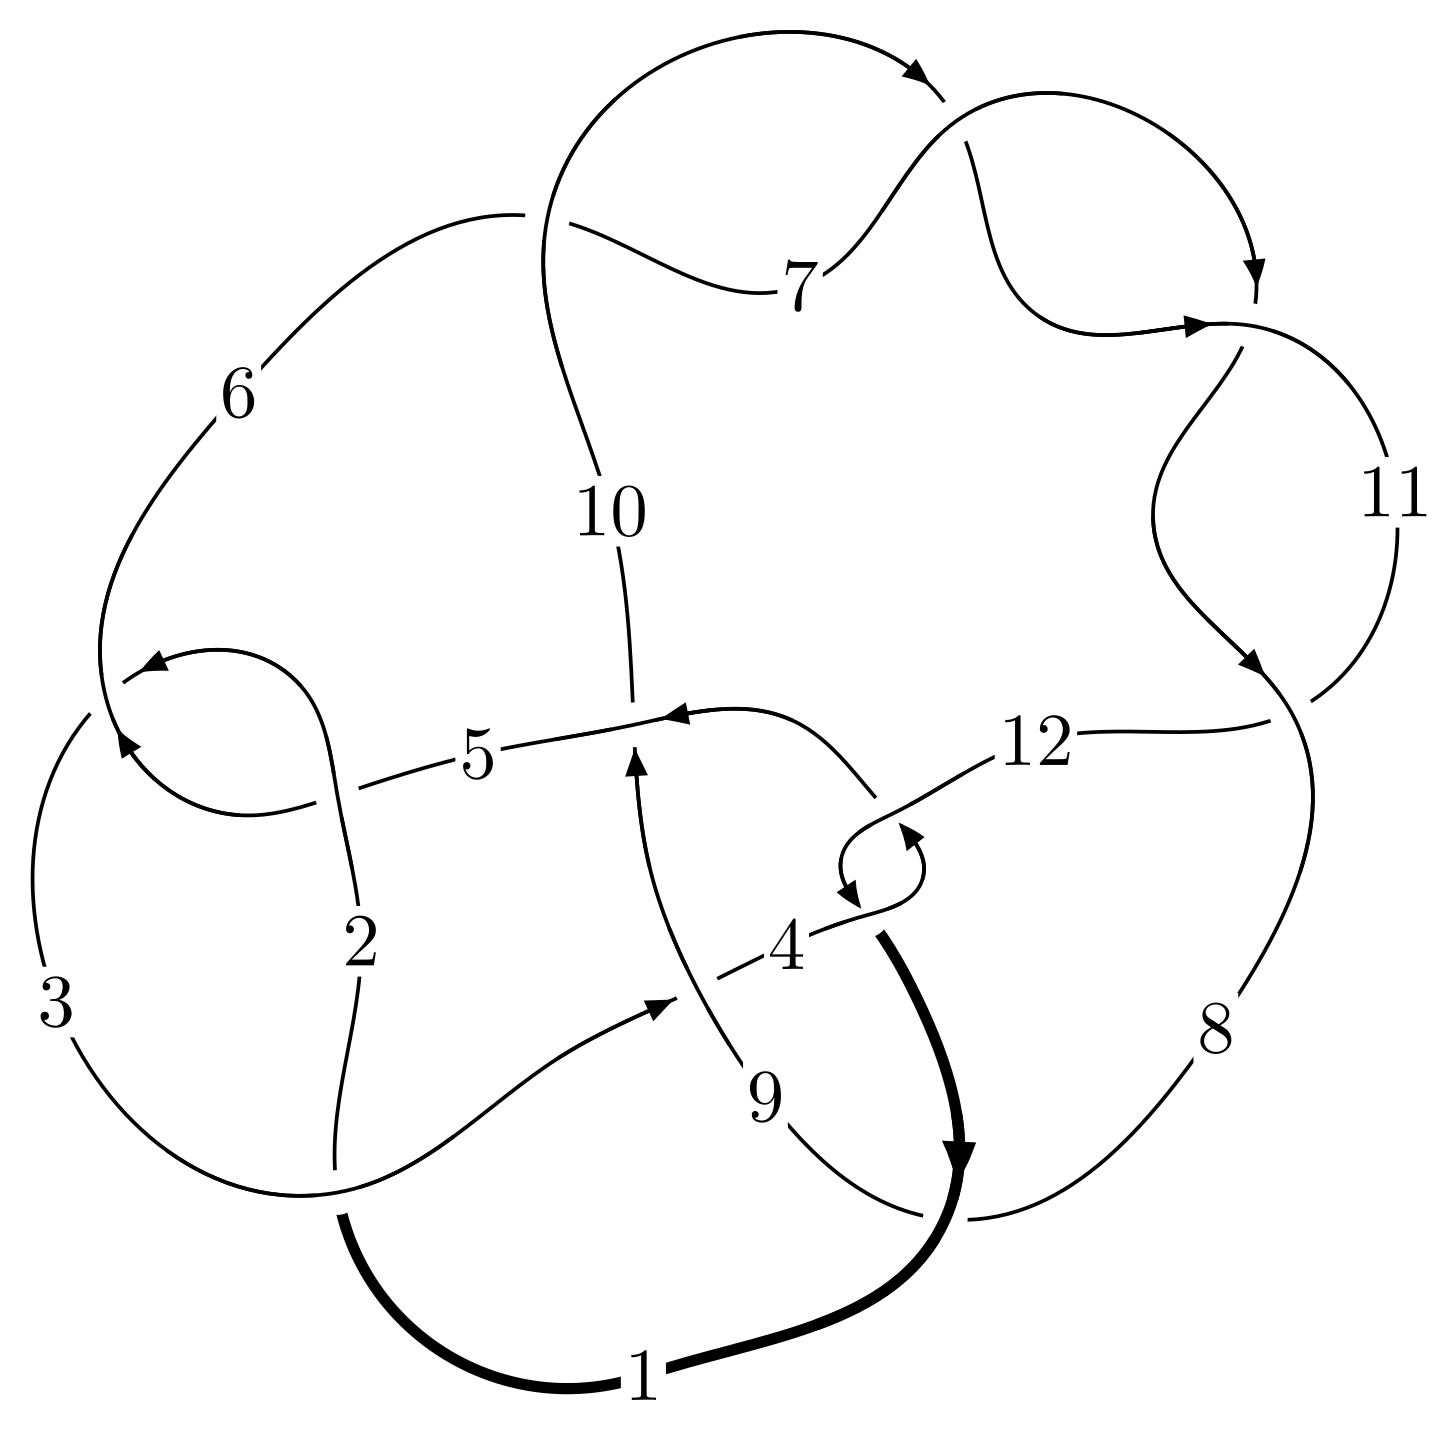
\includegraphics[width=112pt]{../../../GIT/diagram.site/Diagrams/png/1212_12a_0411.png}\\
\ \ \ A knot diagram\footnotemark}&
\allowdisplaybreaks
\textbf{Linearized knot diagam} \\
\cline{2-2}
 &
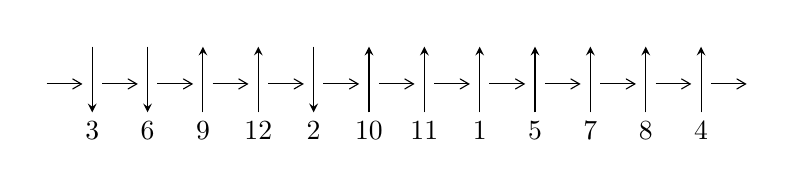
\begin{tikzpicture}[x=20pt, y=17pt]
	% nodes
	\node (C0) at (0, 0) {};
	\node (C1) at (1, 0) {};
	\node (C1U) at (1, +1) {};
	\node (C1D) at (1, -1) {3};

	\node (C2) at (2, 0) {};
	\node (C2U) at (2, +1) {};
	\node (C2D) at (2, -1) {6};

	\node (C3) at (3, 0) {};
	\node (C3U) at (3, +1) {};
	\node (C3D) at (3, -1) {9};

	\node (C4) at (4, 0) {};
	\node (C4U) at (4, +1) {};
	\node (C4D) at (4, -1) {12};

	\node (C5) at (5, 0) {};
	\node (C5U) at (5, +1) {};
	\node (C5D) at (5, -1) {2};

	\node (C6) at (6, 0) {};
	\node (C6U) at (6, +1) {};
	\node (C6D) at (6, -1) {10};

	\node (C7) at (7, 0) {};
	\node (C7U) at (7, +1) {};
	\node (C7D) at (7, -1) {11};

	\node (C8) at (8, 0) {};
	\node (C8U) at (8, +1) {};
	\node (C8D) at (8, -1) {1};

	\node (C9) at (9, 0) {};
	\node (C9U) at (9, +1) {};
	\node (C9D) at (9, -1) {5};

	\node (C10) at (10, 0) {};
	\node (C10U) at (10, +1) {};
	\node (C10D) at (10, -1) {7};

	\node (C11) at (11, 0) {};
	\node (C11U) at (11, +1) {};
	\node (C11D) at (11, -1) {8};

	\node (C12) at (12, 0) {};
	\node (C12U) at (12, +1) {};
	\node (C12D) at (12, -1) {4};
	\node (C13) at (13, 0) {};

	% arrows
	\draw[->,>={angle 60}]
	(C0) edge (C1) (C1) edge (C2) (C2) edge (C3) (C3) edge (C4) (C4) edge (C5) (C5) edge (C6) (C6) edge (C7) (C7) edge (C8) (C8) edge (C9) (C9) edge (C10) (C10) edge (C11) (C11) edge (C12) (C12) edge (C13) ;	\draw[->,>=stealth]
	(C1U) edge (C1D) (C2U) edge (C2D) (C3D) edge (C3U) (C4D) edge (C4U) (C5U) edge (C5D) (C6D) edge (C6U) (C7D) edge (C7U) (C8D) edge (C8U) (C9D) edge (C9U) (C10D) edge (C10U) (C11D) edge (C11U) (C12D) edge (C12U) ;
	\end{tikzpicture} \\
\hhline{~~} \\& 
\textbf{Solving Sequence} \\ \cline{2-2} 
 &
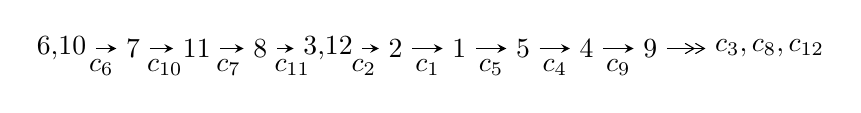
\begin{tikzpicture}[x=23pt, y=7pt]
	% node
	\node (A0) at (-1/8, 0) {6,10};
	\node (A1) at (1, 0) {7};
	\node (A2) at (2, 0) {11};
	\node (A3) at (3, 0) {8};
	\node (A4) at (65/16, 0) {3,12};
	\node (A5) at (41/8, 0) {2};
	\node (A6) at (49/8, 0) {1};
	\node (A7) at (57/8, 0) {5};
	\node (A8) at (65/8, 0) {4};
	\node (A9) at (73/8, 0) {9};
	\node (C1) at (1/2, -1) {$c_{6}$};
	\node (C2) at (3/2, -1) {$c_{10}$};
	\node (C3) at (5/2, -1) {$c_{7}$};
	\node (C4) at (7/2, -1) {$c_{11}$};
	\node (C5) at (37/8, -1) {$c_{2}$};
	\node (C6) at (45/8, -1) {$c_{1}$};
	\node (C7) at (53/8, -1) {$c_{5}$};
	\node (C8) at (61/8, -1) {$c_{4}$};
	\node (C9) at (69/8, -1) {$c_{9}$};
	\node (A10) at (11, 0) {$c_{3},c_{8},c_{12}$};

	% edge
	\draw[->,>=stealth]	
	(A0) edge (A1) (A1) edge (A2) (A2) edge (A3) (A3) edge (A4) (A4) edge (A5) (A5) edge (A6) (A6) edge (A7) (A7) edge (A8) (A8) edge (A9) ;
	\draw[->>,>={angle 60}]	
	(A9) edge (A10);
\end{tikzpicture} \\ 

\end{tabular} \\

\footnotetext{
The image of knot diagram is generated by the software ``\textbf{Draw programme}" developed by Andrew Bartholomew(\url{http://www.layer8.co.uk/maths/draw/index.htm\#Running-draw}), where we modified some parts for our purpose(\url{https://github.com/CATsTAILs/LinksPainter}).
}\phantom \\ \newline 
\centering \textbf{Ideals for irreducible components\footnotemark of $X_{\text{par}}$} 
 
\begin{align*}
I^u_{1}&=\langle 
-6.05318\times10^{105} u^{79}-2.71139\times10^{106} u^{78}+\cdots+6.14360\times10^{104} b+1.09875\times10^{106},\\
\phantom{I^u_{1}}&\phantom{= \langle  }1.04172\times10^{107} u^{79}+4.58247\times10^{107} u^{78}+\cdots+3.07180\times10^{104} a-1.70407\times10^{107},\;u^{80}+5 u^{79}+\cdots-6 u-1\rangle \\
I^u_{2}&=\langle 
a^2+6 b+4 a+4,\;a^4+2 a^3+6 a^2-4 a+4,\;u+1\rangle \\
\\
\end{align*}
\raggedright * 2 irreducible components of $\dim_{\mathbb{C}}=0$, with total 84 representations.\\
\footnotetext{All coefficients of polynomials are rational numbers. But the coefficients are sometimes approximated in decimal forms when there is not enough margin.}
\newpage
\renewcommand{\arraystretch}{1}
\centering \section*{I. $I^u_{1}= \langle -6.05\times10^{105} u^{79}-2.71\times10^{106} u^{78}+\cdots+6.14\times10^{104} b+1.10\times10^{106},\;1.04\times10^{107} u^{79}+4.58\times10^{107} u^{78}+\cdots+3.07\times10^{104} a-1.70\times10^{107},\;u^{80}+5 u^{79}+\cdots-6 u-1 \rangle$}
\flushleft \textbf{(i) Arc colorings}\\
\begin{tabular}{m{7pt} m{180pt} m{7pt} m{180pt} }
\flushright $a_{6}=$&$\begin{pmatrix}1\\0\end{pmatrix}$ \\
\flushright $a_{10}=$&$\begin{pmatrix}0\\u\end{pmatrix}$ \\
\flushright $a_{7}=$&$\begin{pmatrix}1\\- u^2\end{pmatrix}$ \\
\flushright $a_{11}=$&$\begin{pmatrix}u\\- u^3+u\end{pmatrix}$ \\
\flushright $a_{8}=$&$\begin{pmatrix}- u^2+1\\u^4-2 u^2\end{pmatrix}$ \\
\flushright $a_{3}=$&$\begin{pmatrix}-339.123 u^{79}-1491.79 u^{78}+\cdots+2436.78 u+554.746\\9.85281 u^{79}+44.1335 u^{78}+\cdots-72.3996 u-17.8844\end{pmatrix}$ \\
\flushright $a_{12}=$&$\begin{pmatrix}- u^3+2 u\\u^5-3 u^3+u\end{pmatrix}$ \\
\flushright $a_{2}=$&$\begin{pmatrix}-329.270 u^{79}-1447.65 u^{78}+\cdots+2364.38 u+536.861\\9.85281 u^{79}+44.1335 u^{78}+\cdots-72.3996 u-17.8844\end{pmatrix}$ \\
\flushright $a_{1}=$&$\begin{pmatrix}-405.884 u^{79}-1783.77 u^{78}+\cdots+2936.77 u+667.230\\-9.50049 u^{79}-43.5798 u^{78}+\cdots+69.1784 u+16.0314\end{pmatrix}$ \\
\flushright $a_{5}=$&$\begin{pmatrix}142.976 u^{79}+628.242 u^{78}+\cdots-1036.69 u-240.087\\-19.2570 u^{79}-82.9318 u^{78}+\cdots+136.175 u+30.0287\end{pmatrix}$ \\
\flushright $a_{4}=$&$\begin{pmatrix}164.052 u^{79}+719.781 u^{78}+\cdots-1187.59 u-274.887\\-18.4406 u^{79}-79.7156 u^{78}+\cdots+130.155 u+28.5642\end{pmatrix}$ \\
\flushright $a_{9}=$&$\begin{pmatrix}-3509.05 u^{79}-15418.0 u^{78}+\cdots+25205.3 u+5785.93\\176.743 u^{79}+775.971 u^{78}+\cdots-1267.41 u-292.353\end{pmatrix}$\\&\end{tabular}
\flushleft \textbf{(ii) Obstruction class $= -1$}\\~\\
\flushleft \textbf{(iii) Cusp Shapes $= -219.391 u^{79}-967.071 u^{78}+\cdots+1569.64 u+365.051$}\\~\\
\newpage\renewcommand{\arraystretch}{1}
\flushleft \textbf{(iv) u-Polynomials at the component}\newline \\
\begin{tabular}{m{50pt}|m{274pt}}
Crossings & \hspace{64pt}u-Polynomials at each crossing \\
\hline $$\begin{aligned}c_{1}\end{aligned}$$&$\begin{aligned}
&u^{80}+29 u^{79}+\cdots+13 u+4
\end{aligned}$\\
\hline $$\begin{aligned}c_{2},c_{5}\end{aligned}$$&$\begin{aligned}
&u^{80}+5 u^{79}+\cdots-5 u+2
\end{aligned}$\\
\hline $$\begin{aligned}c_{3}\end{aligned}$$&$\begin{aligned}
&u^{80}- u^{79}+\cdots-10 u-1
\end{aligned}$\\
\hline $$\begin{aligned}c_{4},c_{12}\end{aligned}$$&$\begin{aligned}
&u^{80}+5 u^{79}+\cdots+14 u+1
\end{aligned}$\\
\hline $$\begin{aligned}c_{6},c_{7},c_{10}\\c_{11}\end{aligned}$$&$\begin{aligned}
&u^{80}-5 u^{79}+\cdots+6 u-1
\end{aligned}$\\
\hline $$\begin{aligned}c_{8}\end{aligned}$$&$\begin{aligned}
&u^{80}+7 u^{79}+\cdots-616 u-121
\end{aligned}$\\
\hline $$\begin{aligned}c_{9}\end{aligned}$$&$\begin{aligned}
&u^{80}+15 u^{79}+\cdots-497268 u-29873
\end{aligned}$\\
\hline
\end{tabular}\\~\\
\newpage\renewcommand{\arraystretch}{1}
\flushleft \textbf{(v) Riley Polynomials at the component}\newline \\
\begin{tabular}{m{50pt}|m{274pt}}
Crossings & \hspace{64pt}Riley Polynomials at each crossing \\
\hline $$\begin{aligned}c_{1}\end{aligned}$$&$\begin{aligned}
&y^{80}+47 y^{79}+\cdots-19809 y+16
\end{aligned}$\\
\hline $$\begin{aligned}c_{2},c_{5}\end{aligned}$$&$\begin{aligned}
&y^{80}-29 y^{79}+\cdots-13 y+4
\end{aligned}$\\
\hline $$\begin{aligned}c_{3}\end{aligned}$$&$\begin{aligned}
&y^{80}+9 y^{79}+\cdots-98 y+1
\end{aligned}$\\
\hline $$\begin{aligned}c_{4},c_{12}\end{aligned}$$&$\begin{aligned}
&y^{80}+45 y^{79}+\cdots-134 y+1
\end{aligned}$\\
\hline $$\begin{aligned}c_{6},c_{7},c_{10}\\c_{11}\end{aligned}$$&$\begin{aligned}
&y^{80}-95 y^{79}+\cdots-50 y+1
\end{aligned}$\\
\hline $$\begin{aligned}c_{8}\end{aligned}$$&$\begin{aligned}
&y^{80}+299 y^{79}+\cdots-532400 y+14641
\end{aligned}$\\
\hline $$\begin{aligned}c_{9}\end{aligned}$$&$\begin{aligned}
&y^{80}-321 y^{79}+\cdots-110926727384 y+892396129
\end{aligned}$\\
\hline
\end{tabular}\\~\\
\newpage\flushleft \textbf{(vi) Complex Volumes and Cusp Shapes}
$$\begin{array}{c|c|c}  
\text{Solutions to }I^u_{1}& \I (\text{vol} + \sqrt{-1}CS) & \text{Cusp shape}\\
 \hline 
\begin{aligned}
u &= -0.982239 + 0.110037 I \\
a &= \phantom{-}0.60518 + 1.80389 I \\
b &= -0.832671 - 0.498946 I\end{aligned}
 & \phantom{-}1.69931 - 2.04874 I & \phantom{-0.000000 } 0 \\ \hline\begin{aligned}
u &= -0.982239 - 0.110037 I \\
a &= \phantom{-}0.60518 - 1.80389 I \\
b &= -0.832671 + 0.498946 I\end{aligned}
 & \phantom{-}1.69931 + 2.04874 I & \phantom{-0.000000 } 0 \\ \hline\begin{aligned}
u &= -0.759367 + 0.618307 I \\
a &= -0.344166 + 0.141148 I \\
b &= \phantom{-}0.830140 - 0.649151 I\end{aligned}
 & \phantom{-}2.36183 + 0.48997 I & \phantom{-0.000000 } 0 \\ \hline\begin{aligned}
u &= -0.759367 - 0.618307 I \\
a &= -0.344166 - 0.141148 I \\
b &= \phantom{-}0.830140 + 0.649151 I\end{aligned}
 & \phantom{-}2.36183 - 0.48997 I & \phantom{-0.000000 } 0 \\ \hline\begin{aligned}
u &= \phantom{-}0.874853 + 0.530372 I \\
a &= \phantom{-}0.802361 + 0.585193 I \\
b &= -0.571602 - 0.856402 I\end{aligned}
 & \phantom{-}1.75059 + 7.74311 I & \phantom{-0.000000 } 0 \\ \hline\begin{aligned}
u &= \phantom{-}0.874853 - 0.530372 I \\
a &= \phantom{-}0.802361 - 0.585193 I \\
b &= -0.571602 + 0.856402 I\end{aligned}
 & \phantom{-}1.75059 - 7.74311 I & \phantom{-0.000000 } 0 \\ \hline\begin{aligned}
u &= \phantom{-}0.873797 + 0.412672 I \\
a &= \phantom{-}0.39497 + 1.86274 I \\
b &= \phantom{-}1.069280 - 0.698680 I\end{aligned}
 & \phantom{-}3.64655 + 8.02514 I & \phantom{-0.000000 } 0 \\ \hline\begin{aligned}
u &= \phantom{-}0.873797 - 0.412672 I \\
a &= \phantom{-}0.39497 - 1.86274 I \\
b &= \phantom{-}1.069280 + 0.698680 I\end{aligned}
 & \phantom{-}3.64655 - 8.02514 I & \phantom{-0.000000 } 0 \\ \hline\begin{aligned}
u &= -0.655250 + 0.692019 I \\
a &= \phantom{-}0.86289 - 1.33749 I \\
b &= \phantom{-}0.869750 + 0.660212 I\end{aligned}
 & \phantom{-}2.24057 - 4.60261 I & \phantom{-0.000000 } 0 \\ \hline\begin{aligned}
u &= -0.655250 - 0.692019 I \\
a &= \phantom{-}0.86289 + 1.33749 I \\
b &= \phantom{-}0.869750 - 0.660212 I\end{aligned}
 & \phantom{-}2.24057 + 4.60261 I & \phantom{-0.000000 } 0\\
 \hline 
 \end{array}$$\newpage$$\begin{array}{c|c|c}  
\text{Solutions to }I^u_{1}& \I (\text{vol} + \sqrt{-1}CS) & \text{Cusp shape}\\
 \hline 
\begin{aligned}
u &= \phantom{-}0.862986 + 0.606936 I \\
a &= -0.60152 - 1.82721 I \\
b &= -1.072300 + 0.693311 I\end{aligned}
 & \phantom{-}0.23574 + 13.50530 I & \phantom{-0.000000 } 0 \\ \hline\begin{aligned}
u &= \phantom{-}0.862986 - 0.606936 I \\
a &= -0.60152 + 1.82721 I \\
b &= -1.072300 - 0.693311 I\end{aligned}
 & \phantom{-}0.23574 - 13.50530 I & \phantom{-0.000000 } 0 \\ \hline\begin{aligned}
u &= \phantom{-}0.890674 + 0.278765 I \\
a &= -0.775206 - 0.805171 I \\
b &= \phantom{-}0.569460 + 0.870192 I\end{aligned}
 & \phantom{-}5.15281 + 2.22250 I & \phantom{-0.000000 } 0 \\ \hline\begin{aligned}
u &= \phantom{-}0.890674 - 0.278765 I \\
a &= -0.775206 + 0.805171 I \\
b &= \phantom{-}0.569460 - 0.870192 I\end{aligned}
 & \phantom{-}5.15281 - 2.22250 I & \phantom{-0.000000 } 0 \\ \hline\begin{aligned}
u &= -1.001950 + 0.553061 I \\
a &= -0.32963 + 1.53584 I \\
b &= -0.763637 - 0.645618 I\end{aligned}
 & \phantom{-}2.03589 - 1.14374 I & \phantom{-0.000000 } 0 \\ \hline\begin{aligned}
u &= -1.001950 - 0.553061 I \\
a &= -0.32963 - 1.53584 I \\
b &= -0.763637 + 0.645618 I\end{aligned}
 & \phantom{-}2.03589 + 1.14374 I & \phantom{-0.000000 } 0 \\ \hline\begin{aligned}
u &= \phantom{-}0.086726 + 0.850018 I \\
a &= -0.681133 + 0.501362 I \\
b &= -1.019290 - 0.654420 I\end{aligned}
 & -2.13020 - 8.69514 I & \phantom{-0.000000 } 0 \\ \hline\begin{aligned}
u &= \phantom{-}0.086726 - 0.850018 I \\
a &= -0.681133 - 0.501362 I \\
b &= -1.019290 + 0.654420 I\end{aligned}
 & -2.13020 + 8.69514 I & \phantom{-0.000000 } 0 \\ \hline\begin{aligned}
u &= \phantom{-}0.673885 + 0.494383 I \\
a &= \phantom{-}0.633666 + 0.692030 I \\
b &= \phantom{-}1.176500 - 0.080914 I\end{aligned}
 & -4.82659 + 6.36458 I & \phantom{-0.000000 } 0 \\ \hline\begin{aligned}
u &= \phantom{-}0.673885 - 0.494383 I \\
a &= \phantom{-}0.633666 - 0.692030 I \\
b &= \phantom{-}1.176500 + 0.080914 I\end{aligned}
 & -4.82659 - 6.36458 I & \phantom{-0.000000 } 0\\
 \hline 
 \end{array}$$\newpage$$\begin{array}{c|c|c}  
\text{Solutions to }I^u_{1}& \I (\text{vol} + \sqrt{-1}CS) & \text{Cusp shape}\\
 \hline 
\begin{aligned}
u &= -0.731433 + 0.268270 I \\
a &= \phantom{-}0.380165 + 0.677378 I \\
b &= \phantom{-}0.017151 + 0.232479 I\end{aligned}
 & \phantom{-}0.144692 - 0.492251 I & \phantom{-0.000000 } 0 \\ \hline\begin{aligned}
u &= -0.731433 - 0.268270 I \\
a &= \phantom{-}0.380165 - 0.677378 I \\
b &= \phantom{-}0.017151 - 0.232479 I\end{aligned}
 & \phantom{-}0.144692 + 0.492251 I & \phantom{-0.000000 } 0 \\ \hline\begin{aligned}
u &= \phantom{-}0.000926 + 0.775832 I \\
a &= -0.416848 - 0.459903 I \\
b &= -0.600120 + 0.713934 I\end{aligned}
 & -0.90150 - 3.42282 I & \phantom{-0.000000 } 0 \\ \hline\begin{aligned}
u &= \phantom{-}0.000926 - 0.775832 I \\
a &= -0.416848 + 0.459903 I \\
b &= -0.600120 - 0.713934 I\end{aligned}
 & -0.90150 + 3.42282 I & \phantom{-0.000000 } 0 \\ \hline\begin{aligned}
u &= -1.127500 + 0.540430 I \\
a &= \phantom{-}0.446319 - 0.595511 I \\
b &= -0.930935 + 0.641996 I\end{aligned}
 & \phantom{-}1.51642 + 3.88958 I & \phantom{-0.000000 } 0 \\ \hline\begin{aligned}
u &= -1.127500 - 0.540430 I \\
a &= \phantom{-}0.446319 + 0.595511 I \\
b &= -0.930935 - 0.641996 I\end{aligned}
 & \phantom{-}1.51642 - 3.88958 I & \phantom{-0.000000 } 0 \\ \hline\begin{aligned}
u &= \phantom{-}0.705170 + 0.221551 I \\
a &= \phantom{-}0.143659 - 1.137600 I \\
b &= -0.379959 + 0.898795 I\end{aligned}
 & \phantom{-}0.71940 + 3.75775 I & \phantom{-}6.00000 - 11.49284 I \\ \hline\begin{aligned}
u &= \phantom{-}0.705170 - 0.221551 I \\
a &= \phantom{-}0.143659 + 1.137600 I \\
b &= -0.379959 - 0.898795 I\end{aligned}
 & \phantom{-}0.71940 - 3.75775 I & \phantom{-}6.00000 + 11.49284 I \\ \hline\begin{aligned}
u &= -1.272480 + 0.232109 I \\
a &= -0.077573 - 1.327820 I \\
b &= \phantom{-}0.862974 + 0.150904 I\end{aligned}
 & -1.44152 - 0.51003 I & \phantom{-0.000000 } 0 \\ \hline\begin{aligned}
u &= -1.272480 - 0.232109 I \\
a &= -0.077573 + 1.327820 I \\
b &= \phantom{-}0.862974 - 0.150904 I\end{aligned}
 & -1.44152 + 0.51003 I & \phantom{-0.000000 } 0\\
 \hline 
 \end{array}$$\newpage$$\begin{array}{c|c|c}  
\text{Solutions to }I^u_{1}& \I (\text{vol} + \sqrt{-1}CS) & \text{Cusp shape}\\
 \hline 
\begin{aligned}
u &= \phantom{-}0.243048 + 0.629200 I \\
a &= \phantom{-}1.17488 + 1.11461 I \\
b &= \phantom{-}1.061150 - 0.014230 I\end{aligned}
 & -6.12935 - 2.55225 I & -1.74573 + 1.31196 I \\ \hline\begin{aligned}
u &= \phantom{-}0.243048 - 0.629200 I \\
a &= \phantom{-}1.17488 - 1.11461 I \\
b &= \phantom{-}1.061150 + 0.014230 I\end{aligned}
 & -6.12935 + 2.55225 I & -1.74573 - 1.31196 I \\ \hline\begin{aligned}
u &= -0.111177 + 0.623613 I \\
a &= \phantom{-}1.101240 - 0.355446 I \\
b &= \phantom{-}0.975206 + 0.620136 I\end{aligned}
 & \phantom{-}0.69805 - 4.57533 I & \phantom{-}7.44408 + 5.23824 I \\ \hline\begin{aligned}
u &= -0.111177 - 0.623613 I \\
a &= \phantom{-}1.101240 + 0.355446 I \\
b &= \phantom{-}0.975206 - 0.620136 I\end{aligned}
 & \phantom{-}0.69805 + 4.57533 I & \phantom{-}7.44408 - 5.23824 I \\ \hline\begin{aligned}
u &= -0.310855 + 0.540574 I \\
a &= \phantom{-}0.484610 - 0.177259 I \\
b &= \phantom{-}0.699014 - 0.609698 I\end{aligned}
 & \phantom{-}1.56224 + 0.31078 I & \phantom{-}10.32905 - 0.04232 I \\ \hline\begin{aligned}
u &= -0.310855 - 0.540574 I \\
a &= \phantom{-}0.484610 + 0.177259 I \\
b &= \phantom{-}0.699014 + 0.609698 I\end{aligned}
 & \phantom{-}1.56224 - 0.31078 I & \phantom{-}10.32905 + 0.04232 I \\ \hline\begin{aligned}
u &= -0.604081 + 0.001377 I \\
a &= \phantom{-}13.5746 - 17.1139 I \\
b &= \phantom{-}0.877405 + 0.507465 I\end{aligned}
 & -0.68319 - 2.03117 I & \phantom{-}157.990 - 13.051 I \\ \hline\begin{aligned}
u &= -0.604081 - 0.001377 I \\
a &= \phantom{-}13.5746 + 17.1139 I \\
b &= \phantom{-}0.877405 - 0.507465 I\end{aligned}
 & -0.68319 + 2.03117 I & \phantom{-}157.990 + 13.051 I \\ \hline\begin{aligned}
u &= \phantom{-}0.540486 + 0.177581 I \\
a &= \phantom{-}0.36709 - 2.47230 I \\
b &= -1.008760 + 0.761264 I\end{aligned}
 & -1.52216 + 3.07297 I & -0.13001 - 12.94551 I \\ \hline\begin{aligned}
u &= \phantom{-}0.540486 - 0.177581 I \\
a &= \phantom{-}0.36709 + 2.47230 I \\
b &= -1.008760 - 0.761264 I\end{aligned}
 & -1.52216 - 3.07297 I & -0.13001 + 12.94551 I\\
 \hline 
 \end{array}$$\newpage$$\begin{array}{c|c|c}  
\text{Solutions to }I^u_{1}& \I (\text{vol} + \sqrt{-1}CS) & \text{Cusp shape}\\
 \hline 
\begin{aligned}
u &= -0.452044\phantom{ +0.000000I} \\
a &= \phantom{-}0.820522\phantom{ +0.000000I} \\
b &= \phantom{-}0.201146\phantom{ +0.000000I}\end{aligned}
 & \phantom{-}0.707924\phantom{ +0.000000I} & \phantom{-}14.1880\phantom{ +0.000000I} \\ \hline\begin{aligned}
u &= \phantom{-}1.54810 + 0.07689 I \\
a &= -0.806628 + 0.115866 I \\
b &= -0.972871 + 0.136497 I\end{aligned}
 & \phantom{-}5.02760 + 3.22521 I & \phantom{-0.000000 } 0 \\ \hline\begin{aligned}
u &= \phantom{-}1.54810 - 0.07689 I \\
a &= -0.806628 - 0.115866 I \\
b &= -0.972871 - 0.136497 I\end{aligned}
 & \phantom{-}5.02760 - 3.22521 I & \phantom{-0.000000 } 0 \\ \hline\begin{aligned}
u &= \phantom{-}0.357453 + 0.272374 I \\
a &= -0.28354 - 1.47622 I \\
b &= -1.082900 + 0.195290 I\end{aligned}
 & -1.99021 + 1.12837 I & -0.61556 - 4.33419 I \\ \hline\begin{aligned}
u &= \phantom{-}0.357453 - 0.272374 I \\
a &= -0.28354 + 1.47622 I \\
b &= -1.082900 - 0.195290 I\end{aligned}
 & -1.99021 - 1.12837 I & -0.61556 + 4.33419 I \\ \hline\begin{aligned}
u &= \phantom{-}1.57162\phantom{ +0.000000I} \\
a &= \phantom{-}0.420961\phantom{ +0.000000I} \\
b &= \phantom{-}0.775180\phantom{ +0.000000I}\end{aligned}
 & \phantom{-}7.67792\phantom{ +0.000000I} & \phantom{-0.000000 } 0 \\ \hline\begin{aligned}
u &= -1.57728 + 0.00721 I \\
a &= \phantom{-}0.560042 + 0.801944 I \\
b &= -1.37891 - 0.39634 I\end{aligned}
 & \phantom{-}4.86129 - 1.42349 I & \phantom{-0.000000 } 0 \\ \hline\begin{aligned}
u &= -1.57728 - 0.00721 I \\
a &= \phantom{-}0.560042 - 0.801944 I \\
b &= -1.37891 + 0.39634 I\end{aligned}
 & \phantom{-}4.86129 + 1.42349 I & \phantom{-0.000000 } 0 \\ \hline\begin{aligned}
u &= -1.59511 + 0.02885 I \\
a &= \phantom{-}0.80382 + 1.88339 I \\
b &= -1.05746 - 0.93966 I\end{aligned}
 & \phantom{-}5.96830 - 3.68106 I & \phantom{-0.000000 } 0 \\ \hline\begin{aligned}
u &= -1.59511 - 0.02885 I \\
a &= \phantom{-}0.80382 - 1.88339 I \\
b &= -1.05746 + 0.93966 I\end{aligned}
 & \phantom{-}5.96830 + 3.68106 I & \phantom{-0.000000 } 0\\
 \hline 
 \end{array}$$\newpage$$\begin{array}{c|c|c}  
\text{Solutions to }I^u_{1}& \I (\text{vol} + \sqrt{-1}CS) & \text{Cusp shape}\\
 \hline 
\begin{aligned}
u &= -0.209332 + 0.339332 I \\
a &= -0.70138 - 2.09676 I \\
b &= -0.567508 - 0.324974 I\end{aligned}
 & -1.43343 - 2.05795 I & \phantom{-}2.20961 + 4.63586 I \\ \hline\begin{aligned}
u &= -0.209332 - 0.339332 I \\
a &= -0.70138 + 2.09676 I \\
b &= -0.567508 + 0.324974 I\end{aligned}
 & -1.43343 + 2.05795 I & \phantom{-}2.20961 - 4.63586 I \\ \hline\begin{aligned}
u &= -1.59909 + 0.12620 I \\
a &= -0.154490 - 0.604773 I \\
b &= \phantom{-}1.277360 + 0.151788 I\end{aligned}
 & \phantom{-}2.88077 - 8.60117 I & \phantom{-0.000000 } 0 \\ \hline\begin{aligned}
u &= -1.59909 - 0.12620 I \\
a &= -0.154490 + 0.604773 I \\
b &= \phantom{-}1.277360 - 0.151788 I\end{aligned}
 & \phantom{-}2.88077 + 8.60117 I & \phantom{-0.000000 } 0 \\ \hline\begin{aligned}
u &= \phantom{-}1.60983 + 0.00290 I \\
a &= \phantom{-}1.69153 + 4.69097 I \\
b &= \phantom{-}0.914469 - 0.540849 I\end{aligned}
 & \phantom{-}7.10700 + 2.05661 I & \phantom{-0.000000 } 0 \\ \hline\begin{aligned}
u &= \phantom{-}1.60983 - 0.00290 I \\
a &= \phantom{-}1.69153 - 4.69097 I \\
b &= \phantom{-}0.914469 + 0.540849 I\end{aligned}
 & \phantom{-}7.10700 - 2.05661 I & \phantom{-0.000000 } 0 \\ \hline\begin{aligned}
u &= -1.62146 + 0.05130 I \\
a &= \phantom{-}0.25483 + 1.52795 I \\
b &= -0.314660 - 1.105270 I\end{aligned}
 & \phantom{-}8.79176 - 4.72449 I & \phantom{-0.000000 } 0 \\ \hline\begin{aligned}
u &= -1.62146 - 0.05130 I \\
a &= \phantom{-}0.25483 - 1.52795 I \\
b &= -0.314660 + 1.105270 I\end{aligned}
 & \phantom{-}8.79176 + 4.72449 I & \phantom{-0.000000 } 0 \\ \hline\begin{aligned}
u &= \phantom{-}0.331464 + 0.167817 I \\
a &= \phantom{-}0.790108 + 0.421831 I \\
b &= -1.086350 - 0.487000 I\end{aligned}
 & -2.01483 - 1.42900 I & -2.63503 - 2.24034 I \\ \hline\begin{aligned}
u &= \phantom{-}0.331464 - 0.167817 I \\
a &= \phantom{-}0.790108 - 0.421831 I \\
b &= -1.086350 + 0.487000 I\end{aligned}
 & -2.01483 + 1.42900 I & -2.63503 + 2.24034 I\\
 \hline 
 \end{array}$$\newpage$$\begin{array}{c|c|c}  
\text{Solutions to }I^u_{1}& \I (\text{vol} + \sqrt{-1}CS) & \text{Cusp shape}\\
 \hline 
\begin{aligned}
u &= \phantom{-}1.63729 + 0.04142 I \\
a &= -0.121690 + 0.165881 I \\
b &= \phantom{-}0.186036 - 0.459060 I\end{aligned}
 & \phantom{-}8.44312 + 1.45094 I & \phantom{-0.000000 } 0 \\ \hline\begin{aligned}
u &= \phantom{-}1.63729 - 0.04142 I \\
a &= -0.121690 - 0.165881 I \\
b &= \phantom{-}0.186036 + 0.459060 I\end{aligned}
 & \phantom{-}8.44312 - 1.45094 I & \phantom{-0.000000 } 0 \\ \hline\begin{aligned}
u &= \phantom{-}1.63038 + 0.22067 I \\
a &= \phantom{-}0.09225 + 1.74343 I \\
b &= \phantom{-}0.968177 - 0.699422 I\end{aligned}
 & \phantom{-}9.99013 + 8.08376 I & \phantom{-0.000000 } 0 \\ \hline\begin{aligned}
u &= \phantom{-}1.63038 - 0.22067 I \\
a &= \phantom{-}0.09225 - 1.74343 I \\
b &= \phantom{-}0.968177 + 0.699422 I\end{aligned}
 & \phantom{-}9.99013 - 8.08376 I & \phantom{-0.000000 } 0 \\ \hline\begin{aligned}
u &= -1.66412 + 0.07716 I \\
a &= -0.82132 + 1.36692 I \\
b &= \phantom{-}0.609910 - 1.021180 I\end{aligned}
 & \phantom{-}14.0285 - 3.6133 I & \phantom{-0.000000 } 0 \\ \hline\begin{aligned}
u &= -1.66412 - 0.07716 I \\
a &= -0.82132 - 1.36692 I \\
b &= \phantom{-}0.609910 + 1.021180 I\end{aligned}
 & \phantom{-}14.0285 + 3.6133 I & \phantom{-0.000000 } 0 \\ \hline\begin{aligned}
u &= -1.66410 + 0.11541 I \\
a &= -0.28155 - 1.88460 I \\
b &= \phantom{-}1.119640 + 0.766021 I\end{aligned}
 & \phantom{-}12.4183 - 10.0748 I & \phantom{-0.000000 } 0 \\ \hline\begin{aligned}
u &= -1.66410 - 0.11541 I \\
a &= -0.28155 + 1.88460 I \\
b &= \phantom{-}1.119640 - 0.766021 I\end{aligned}
 & \phantom{-}12.4183 + 10.0748 I & \phantom{-0.000000 } 0 \\ \hline\begin{aligned}
u &= \phantom{-}1.66377 + 0.17561 I \\
a &= -0.762447 - 0.909794 I \\
b &= \phantom{-}0.720008 + 0.743870 I\end{aligned}
 & \phantom{-}10.73520 + 2.58534 I & \phantom{-0.000000 } 0 \\ \hline\begin{aligned}
u &= \phantom{-}1.66377 - 0.17561 I \\
a &= -0.762447 + 0.909794 I \\
b &= \phantom{-}0.720008 - 0.743870 I\end{aligned}
 & \phantom{-}10.73520 - 2.58534 I & \phantom{-0.000000 } 0\\
 \hline 
 \end{array}$$\newpage$$\begin{array}{c|c|c}  
\text{Solutions to }I^u_{1}& \I (\text{vol} + \sqrt{-1}CS) & \text{Cusp shape}\\
 \hline 
\begin{aligned}
u &= -1.66760 + 0.15263 I \\
a &= \phantom{-}0.93902 - 1.16501 I \\
b &= -0.587447 + 0.950346 I\end{aligned}
 & \phantom{-}10.4735 - 10.3982 I & \phantom{-0.000000 } 0 \\ \hline\begin{aligned}
u &= -1.66760 - 0.15263 I \\
a &= \phantom{-}0.93902 + 1.16501 I \\
b &= -0.587447 - 0.950346 I\end{aligned}
 & \phantom{-}10.4735 + 10.3982 I & \phantom{-0.000000 } 0 \\ \hline\begin{aligned}
u &= -1.66703 + 0.17926 I \\
a &= \phantom{-}0.08049 + 1.99128 I \\
b &= -1.106230 - 0.731601 I\end{aligned}
 & \phantom{-}8.8607 - 16.5566 I & \phantom{-0.000000 } 0 \\ \hline\begin{aligned}
u &= -1.66703 - 0.17926 I \\
a &= \phantom{-}0.08049 - 1.99128 I \\
b &= -1.106230 + 0.731601 I\end{aligned}
 & \phantom{-}8.8607 + 16.5566 I & \phantom{-0.000000 } 0 \\ \hline\begin{aligned}
u &= \phantom{-}1.69474 + 0.10689 I \\
a &= \phantom{-}0.26077 - 1.84251 I \\
b &= -0.912299 + 0.690710 I\end{aligned}
 & \phantom{-}11.56300 + 3.48604 I & \phantom{-0.000000 } 0 \\ \hline\begin{aligned}
u &= \phantom{-}1.69474 - 0.10689 I \\
a &= \phantom{-}0.26077 + 1.84251 I \\
b &= -0.912299 - 0.690710 I\end{aligned}
 & \phantom{-}11.56300 - 3.48604 I & \phantom{-0.000000 } 0 \\ \hline\begin{aligned}
u &= \phantom{-}1.72076 + 0.06241 I \\
a &= \phantom{-}0.83025 + 1.28263 I \\
b &= -0.796402 - 0.710069 I\end{aligned}
 & \phantom{-}11.91770 - 1.88395 I & \phantom{-0.000000 } 0 \\ \hline\begin{aligned}
u &= \phantom{-}1.72076 - 0.06241 I \\
a &= \phantom{-}0.83025 - 1.28263 I \\
b &= -0.796402 + 0.710069 I\end{aligned}
 & \phantom{-}11.91770 + 1.88395 I & \phantom{-0.000000 } 0 \\ \hline\begin{aligned}
u &= -0.184682 + 0.116658 I \\
a &= -1.73641 - 5.49293 I \\
b &= -0.749491 - 0.451267 I\end{aligned}
 & -1.42133 - 2.10255 I & \phantom{-}1.91167 + 3.48130 I \\ \hline\begin{aligned}
u &= -0.184682 - 0.116658 I \\
a &= -1.73641 + 5.49293 I \\
b &= -0.749491 + 0.451267 I\end{aligned}
 & -1.42133 + 2.10255 I & \phantom{-}1.91167 - 3.48130 I\\
 \hline 
 \end{array}$$\newpage\newpage\renewcommand{\arraystretch}{1}
\centering \section*{II. $I^u_{2}= \langle a^2+6 b+4 a+4,\;a^4+2 a^3+6 a^2-4 a+4,\;u+1 \rangle$}
\flushleft \textbf{(i) Arc colorings}\\
\begin{tabular}{m{7pt} m{180pt} m{7pt} m{180pt} }
\flushright $a_{6}=$&$\begin{pmatrix}1\\0\end{pmatrix}$ \\
\flushright $a_{10}=$&$\begin{pmatrix}0\\-1\end{pmatrix}$ \\
\flushright $a_{7}=$&$\begin{pmatrix}1\\-1\end{pmatrix}$ \\
\flushright $a_{11}=$&$\begin{pmatrix}-1\\0\end{pmatrix}$ \\
\flushright $a_{8}=$&$\begin{pmatrix}0\\-1\end{pmatrix}$ \\
\flushright $a_{3}=$&$\begin{pmatrix}a\\-\frac{1}{6} a^2-\frac{2}{3} a-\frac{2}{3}\end{pmatrix}$ \\
\flushright $a_{12}=$&$\begin{pmatrix}-1\\1\end{pmatrix}$ \\
\flushright $a_{2}=$&$\begin{pmatrix}-\frac{1}{6} a^2+\frac{1}{3} a-\frac{2}{3}\\-\frac{1}{6} a^2-\frac{2}{3} a-\frac{2}{3}\end{pmatrix}$ \\
\flushright $a_{1}=$&$\begin{pmatrix}-\frac{1}{6} a^3-\frac{1}{6} a^2-\frac{2}{3} a\\\frac{1}{6} a^3+\frac{1}{6} a^2+\frac{2}{3} a-1\end{pmatrix}$ \\
\flushright $a_{5}=$&$\begin{pmatrix}\frac{1}{6} a^2-\frac{1}{3} a+\frac{2}{3}\\-\frac{1}{6} a^3-\frac{1}{2} a^2- a-\frac{1}{3}\end{pmatrix}$ \\
\flushright $a_{4}=$&$\begin{pmatrix}\frac{1}{6} a^3+\frac{1}{2} a^2+a+\frac{1}{3}\\-\frac{1}{3} a^3-\frac{5}{6} a^2-\frac{7}{3} a\end{pmatrix}$ \\
\flushright $a_{9}=$&$\begin{pmatrix}-\frac{1}{6} a^3+\frac{1}{6} a^2-\frac{1}{3} a+\frac{1}{3}\\-\frac{1}{3} a^2-\frac{1}{3} a-\frac{4}{3}\end{pmatrix}$\\&\end{tabular}
\flushleft \textbf{(ii) Obstruction class $= 1$}\\~\\
\flushleft \textbf{(iii) Cusp Shapes $= \frac{2}{3} a^3+2 a^2+4 a+\frac{16}{3}$}\\~\\
\newpage\renewcommand{\arraystretch}{1}
\flushleft \textbf{(iv) u-Polynomials at the component}\newline \\
\begin{tabular}{m{50pt}|m{274pt}}
Crossings & \hspace{64pt}u-Polynomials at each crossing \\
\hline $$\begin{aligned}c_{1}\end{aligned}$$&$\begin{aligned}
&(u^2- u+1)^2
\end{aligned}$\\
\hline $$\begin{aligned}c_{2},c_{5}\end{aligned}$$&$\begin{aligned}
&u^4- u^2+1
\end{aligned}$\\
\hline $$\begin{aligned}c_{3},c_{4},c_{12}\end{aligned}$$&$\begin{aligned}
&(u^2+1)^2
\end{aligned}$\\
\hline $$\begin{aligned}c_{6},c_{7}\end{aligned}$$&$\begin{aligned}
&(u+1)^4
\end{aligned}$\\
\hline $$\begin{aligned}c_{8}\end{aligned}$$&$\begin{aligned}
&u^4+4 u^3+5 u^2+2 u+1
\end{aligned}$\\
\hline $$\begin{aligned}c_{9}\end{aligned}$$&$\begin{aligned}
&u^4-2 u^3+5 u^2-4 u+1
\end{aligned}$\\
\hline $$\begin{aligned}c_{10},c_{11}\end{aligned}$$&$\begin{aligned}
&(u-1)^4
\end{aligned}$\\
\hline
\end{tabular}\\~\\
\newpage\renewcommand{\arraystretch}{1}
\flushleft \textbf{(v) Riley Polynomials at the component}\newline \\
\begin{tabular}{m{50pt}|m{274pt}}
Crossings & \hspace{64pt}Riley Polynomials at each crossing \\
\hline $$\begin{aligned}c_{1}\end{aligned}$$&$\begin{aligned}
&(y^2+y+1)^2
\end{aligned}$\\
\hline $$\begin{aligned}c_{2},c_{5}\end{aligned}$$&$\begin{aligned}
&(y^2- y+1)^2
\end{aligned}$\\
\hline $$\begin{aligned}c_{3},c_{4},c_{12}\end{aligned}$$&$\begin{aligned}
&(y+1)^4
\end{aligned}$\\
\hline $$\begin{aligned}c_{6},c_{7},c_{10}\\c_{11}\end{aligned}$$&$\begin{aligned}
&(y-1)^4
\end{aligned}$\\
\hline $$\begin{aligned}c_{8}\end{aligned}$$&$\begin{aligned}
&y^4-6 y^3+11 y^2+6 y+1
\end{aligned}$\\
\hline $$\begin{aligned}c_{9}\end{aligned}$$&$\begin{aligned}
&y^4+6 y^3+11 y^2-6 y+1
\end{aligned}$\\
\hline
\end{tabular}\\~\\
\newpage\flushleft \textbf{(vi) Complex Volumes and Cusp Shapes}
$$\begin{array}{c|c|c}  
\text{Solutions to }I^u_{2}& \I (\text{vol} + \sqrt{-1}CS) & \text{Cusp shape}\\
 \hline 
\begin{aligned}
u &= -1.00000\phantom{ +0.000000I} \\
a &= \phantom{-}0.366025 + 0.633975 I \\
b &= -0.866025 - 0.500000 I\end{aligned}
 & \phantom{-0.000000 } -2.02988 I & \phantom{-}6.00000 + 3.46410 I \\ \hline\begin{aligned}
u &= -1.00000\phantom{ +0.000000I} \\
a &= \phantom{-}0.366025 - 0.633975 I \\
b &= -0.866025 + 0.500000 I\end{aligned}
 & \phantom{-0.000000 -}2.02988 I & \phantom{-}6.00000 - 3.46410 I \\ \hline\begin{aligned}
u &= -1.00000\phantom{ +0.000000I} \\
a &= -1.36603 + 2.36603 I \\
b &= \phantom{-}0.866025 - 0.500000 I\end{aligned}
 & \phantom{-0.000000 -}2.02988 I & \phantom{-}6.00000 - 3.46410 I \\ \hline\begin{aligned}
u &= -1.00000\phantom{ +0.000000I} \\
a &= -1.36603 - 2.36603 I \\
b &= \phantom{-}0.866025 + 0.500000 I\end{aligned}
 & \phantom{-0.000000 } -2.02988 I & \phantom{-}6.00000 + 3.46410 I\\
 \hline 
 \end{array}$$\newpage
\newpage\renewcommand{\arraystretch}{1}
\centering \section*{ III. u-Polynomials}
\begin{tabular}{m{50pt}|m{274pt}}
Crossings & \hspace{64pt}u-Polynomials at each crossing \\
\hline $$\begin{aligned}c_{1}\end{aligned}$$&$\begin{aligned}
&((u^2- u+1)^2)(u^{80}+29 u^{79}+\cdots+13 u+4)
\end{aligned}$\\
\hline $$\begin{aligned}c_{2},c_{5}\end{aligned}$$&$\begin{aligned}
&(u^4- u^2+1)(u^{80}+5 u^{79}+\cdots-5 u+2)
\end{aligned}$\\
\hline $$\begin{aligned}c_{3}\end{aligned}$$&$\begin{aligned}
&((u^2+1)^2)(u^{80}- u^{79}+\cdots-10 u-1)
\end{aligned}$\\
\hline $$\begin{aligned}c_{4},c_{12}\end{aligned}$$&$\begin{aligned}
&((u^2+1)^2)(u^{80}+5 u^{79}+\cdots+14 u+1)
\end{aligned}$\\
\hline $$\begin{aligned}c_{6},c_{7}\end{aligned}$$&$\begin{aligned}
&((u+1)^4)(u^{80}-5 u^{79}+\cdots+6 u-1)
\end{aligned}$\\
\hline $$\begin{aligned}c_{8}\end{aligned}$$&$\begin{aligned}
&(u^4+4 u^3+5 u^2+2 u+1)(u^{80}+7 u^{79}+\cdots-616 u-121)
\end{aligned}$\\
\hline $$\begin{aligned}c_{9}\end{aligned}$$&$\begin{aligned}
&(u^4-2 u^3+5 u^2-4 u+1)(u^{80}+15 u^{79}+\cdots-497268 u-29873)
\end{aligned}$\\
\hline $$\begin{aligned}c_{10},c_{11}\end{aligned}$$&$\begin{aligned}
&((u-1)^4)(u^{80}-5 u^{79}+\cdots+6 u-1)
\end{aligned}$\\
\hline
\end{tabular}\newpage\renewcommand{\arraystretch}{1}
\centering \section*{ IV. Riley Polynomials}
\begin{tabular}{m{50pt}|m{274pt}}
Crossings & \hspace{64pt}Riley Polynomials at each crossing \\
\hline $$\begin{aligned}c_{1}\end{aligned}$$&$\begin{aligned}
&((y^2+y+1)^2)(y^{80}+47 y^{79}+\cdots-19809 y+16)
\end{aligned}$\\
\hline $$\begin{aligned}c_{2},c_{5}\end{aligned}$$&$\begin{aligned}
&((y^2- y+1)^2)(y^{80}-29 y^{79}+\cdots-13 y+4)
\end{aligned}$\\
\hline $$\begin{aligned}c_{3}\end{aligned}$$&$\begin{aligned}
&((y+1)^4)(y^{80}+9 y^{79}+\cdots-98 y+1)
\end{aligned}$\\
\hline $$\begin{aligned}c_{4},c_{12}\end{aligned}$$&$\begin{aligned}
&((y+1)^4)(y^{80}+45 y^{79}+\cdots-134 y+1)
\end{aligned}$\\
\hline $$\begin{aligned}c_{6},c_{7},c_{10}\\c_{11}\end{aligned}$$&$\begin{aligned}
&((y-1)^4)(y^{80}-95 y^{79}+\cdots-50 y+1)
\end{aligned}$\\
\hline $$\begin{aligned}c_{8}\end{aligned}$$&$\begin{aligned}
&(y^4-6 y^3+11 y^2+6 y+1)(y^{80}+299 y^{79}+\cdots-532400 y+14641)
\end{aligned}$\\
\hline $$\begin{aligned}c_{9}\end{aligned}$$&$\begin{aligned}
&(y^4+6 y^3+11 y^2-6 y+1)\\
&\cdot(y^{80}-321 y^{79}+\cdots-110926727384 y+892396129)
\end{aligned}$\\
\hline
\end{tabular}
\vskip 2pc
\end{document}